\documentclass[11pt,a4paper]{article}
% Derivative of HCMUT_RP_template/SoftEng_252/main.tex; original is untouched.
\usepackage[utf8]{vntex}
\usepackage[a4paper,left=25mm,right=23mm,top=28mm,bottom=25mm,headheight=38pt,headsep=12pt]{geometry}
\usepackage{amsmath,amssymb,graphicx,array,booktabs,longtable,tabularx}
\usepackage{fancyhdr,lastpage,xcolor,listings,caption,enumitem}
\usepackage[unicode,colorlinks=true,linkcolor=black,citecolor=blue!50!black,urlcolor=blue!60!black,breaklinks=true]{hyperref}
\usepackage{xurl}
% Shared cover metadata supplied by the two authors.
\newcommand{\AuthorNameOne}{Phạm Duy Anh - 2310139}
\newcommand{\AuthorNameTwo}{Nguyễn Phan Tuấn Duy - 2310491}
\newcommand{\AuthorName}{\AuthorNameOne; \AuthorNameTwo}
\newcommand{\CourseCode}{CO5085}
\newcommand{\CourseName}{Học sâu và ứng dụng trong thị giác máy tính}
\newcommand{\Semester}{Học kỳ 261 -- Năm học 2026--2027}
\newcommand{\AdvisorOne}{TS. Lê Thành Sách}
\newcommand{\AdvisorTwo}{TS. Nguyễn Quốc Minh}
\newcommand{\ReportDate}{Tháng 11 năm 2026}

\graphicspath{{generated/}{shared/}}
\definecolor{hcmut}{RGB}{0,78,137}
\pagestyle{fancy}\fancyhf{}
\fancyhead[L]{\begin{tabular}{@{}cl@{}}
\includegraphics[width=8mm]{hcmut.png}&\begin{tabular}{@{}l@{}}\scriptsize\bfseries Trường Đại học Bách Khoa TP.HCM\\\scriptsize Khoa Khoa học và Kỹ thuật Máy tính\end{tabular}\end{tabular}}
\fancyhead[R]{\scriptsize\CourseCode\ -- HK261}
\fancyfoot[L]{\scriptsize CO5085 -- Năm học 2026--2027}
\fancyfoot[R]{\scriptsize Trang \thepage/\pageref{LastPage}}
\renewcommand{\headrulewidth}{.3pt}\renewcommand{\footrulewidth}{.3pt}
\newsavebox{\reporttable}
\setlength{\parindent}{1.2em}\setlength{\parskip}{.35em}
\renewcommand{\arraystretch}{1.18}
\setcounter{tocdepth}{2}
\setlist{nosep,topsep=4pt}
\captionsetup{font=small,labelfont=bf,skip=7pt}
\lstset{language=Python,basicstyle=\footnotesize\ttfamily,keywordstyle=\color{hcmut}\bfseries,commentstyle=\color{black!55},stringstyle=\color{green!35!black},frame=tb,rulecolor=\color{hcmut!40},breaklines=true,columns=fullflexible,keepspaces=true,showstringspaces=false,numbers=left,numberstyle=\tiny\color{black!50},numbersep=7pt,xleftmargin=12pt,tabsize=4}
\emergencystretch=2em
\newcommand{\source}[1]{\par{\footnotesize\textit{Nguồn:} \path{#1}.}\par}
\newcommand{\fig}[4][.92]{\begin{figure}[htbp]\centering\includegraphics[width=#1\linewidth,height=.68\textheight,keepaspectratio]{#2}\caption{#3}\label{fig:#4}\end{figure}}
\newcommand{\reportcover}[2]{%
\hypersetup{pdftitle={#1},pdfauthor={\AuthorName},pdfsubject={CO5085 HK261}}
\begin{titlepage}\begin{center}
ĐẠI HỌC QUỐC GIA THÀNH PHỐ HỒ CHÍ MINH\\
\textbf{TRƯỜNG ĐẠI HỌC BÁCH KHOA}\\
KHOA KHOA HỌC VÀ KỸ THUẬT MÁY TÍNH
\vspace{16mm}\par
\includegraphics[width=3cm]{hcmut.png}\par\vspace{14mm}
{\large\bfseries \CourseCode\ -- \CourseName}\par\vspace{5mm}
\rule{\linewidth}{.6pt}\par\vspace{7mm}
{\LARGE\bfseries\color{hcmut} #1}\par\vspace{5mm}
{\large #2}\par\vspace{7mm}\rule{\linewidth}{.6pt}\par
\vspace{6mm}\Semester\par
\vfill
\begin{tabular}{rl}Giảng viên: & \AdvisorOne\\ &\AdvisorTwo\\Sinh viên 1: &\AuthorNameOne\\Sinh viên 2: &\AuthorNameTwo\end{tabular}
\vfill TP. Hồ Chí Minh, \ReportDate
\end{center}\end{titlepage}
\tableofcontents\clearpage}
\newcommand{\disclosure}{\subsection*{Khai báo sử dụng AI}
AI được sử dụng để hỗ trợ thiết kế giao diện website và trực quan hóa kết quả; nghiên cứu tài liệu, đối chiếu nguồn tham khảo; xây dựng, rà soát và debug mã nguồn; thiết kế cơ chế điều phối huấn luyện song song bằng hai tiến trình trên hai GPU; tổ chức artifact, kiểm tra tính nhất quán và soạn thảo báo cáo LaTeX. Các số đo trong báo cáo được lấy từ artifact và notebook đã chạy, không thay bằng kết quả do AI tự tạo. Hỗ trợ về mã điều phối không đồng nghĩa AI đã thực hiện thêm các lượt huấn luyện mới trong quá trình biên soạn báo cáo.
Hai thành viên chịu trách nhiệm về nội dung và kết quả được trình bày; cần tự rà soát nguồn, kiểm tra mã, hiểu phương pháp và có khả năng giải thích, bảo vệ toàn bộ nội dung trước khi nộp. Việc dùng AI không thay thế các yêu cầu tự thực hiện và hiểu bài trong đề. URL video chưa được cung cấp và không được tự bổ sung.}

\usepackage{float}
\renewcommand{\fig}[4][.92]{\begin{figure}[H]\centering\includegraphics[width=#1\linewidth,height=.68\textheight,keepaspectratio]{#2}\caption{#3}\label{fig:#4}\end{figure}}
\begin{document}
\reportcover{BÁO CÁO ASSIGNMENT 2}{Sinh khuôn mặt anime bằng DCGAN\\Đối chứng DiffAugment và phân tích paper NeurIPS 2020}

\section{Mục tiêu và phạm vi nghiên cứu}\label{sec:scope}
Bài toán là sinh ảnh khuôn mặt anime RGB$64\times 64$ từ latent ngẫu nhiên, không dùng nhãn điều kiện. Hai biến thể có cùng generator/discriminator DCGAN, khác policy augmentation trong đường huấn luyện: baseline không DiffAugment, biến thể còn lại dùng color, translation và cutout. Cùng seed 42, cùng split, khởi tạo, optimizer, EMA và ngân sách 20.000 updates giúp phép so sánh tập trung vào thay đổi này.

Báo cáo gồm phân tích paper DiffAugment~\cite{diffaugment} và thực nghiệm độc lập trên Anime Face Dataset. Đây là áp dụng một ý tưởng phương pháp trong bối cảnh DCGAN/Anime, \emph{không} phải tái lập toàn bộ paper. Các số đo của paper được tách rõ khỏi kết quả nhóm đã lưu; không so trực tiếp FID khác dataset/extractor/protocol như cùng thang chất lượng tuyệt đối.

\begin{table}[htbp]\centering\small\caption{Truy vết yêu cầu từ \texttt{a2\_co5085.md}.}
\begin{tabularx}{\linewidth}{Xl}\toprule Yêu cầu / bằng chứng & Phần\\\midrule
Bài toán tạo sinh, dataset và EDA & \ref{sec:data}\\
Ít nhất hai phương pháp/biến thể có đối chứng & \ref{sec:model}, \ref{sec:training}\\
Paper: động cơ, phương pháp, thí nghiệm và hạn chế & \ref{sec:paper}\\
Protocol FID/KID/IS/precision/recall và chi phí & \ref{sec:metrics}\\
Bảng kết quả, loss, samples và nội suy & \ref{sec:results}--\ref{sec:visual}\\
Nearest neighbors, giới hạn và tái lập & \ref{sec:nearest}, \ref{sec:limits}, \ref{sec:repro}\\
Video thuyết trình & Chưa cung cấp\\\bottomrule\end{tabularx}\end{table}

DiffAugment cải thiện FID từ 298,51 xuống 41,84; recall tăng từ 0 lên 0,0584 nhưng vẫn thấp. Vì vậy kết luận là cải thiện chất lượng và độ phủ \emph{tương đối với baseline}, không phải đã bao phủ tốt toàn phân phối anime.
\disclosure
\clearpage

\section{Dữ liệu, EDA và pipeline}\label{sec:data}
\subsection{Nguồn và attribution}
Nguồn mount của study là Kaggle \texttt{splcher/animefacedataset}~\cite{anime}; manifest ghi attribution tới repository Anime-Face-Dataset~\cite{animeupstream}. Không suy ra quyền tái phân phối hình gốc chỉ từ việc tải được dataset. License note trong manifest yêu cầu kiểm tra metadata Kaggle và quyền từ nguồn gốc; báo cáo không tự gán giấy phép chuẩn. Bộ báo cáo chỉ kèm hình minh họa cần cho phân tích, không đóng gói raw dataset.

\subsection{Audit, dedup và split}
Code đọc từng ảnh, chuyển RGB, lấy kích thước và hash \texttt{SHA256(str(size) + RGBpixels)} trước split. Do đó dedup dựa trên pixel đã giải mã kèm shape, không chỉ hash byte file. Tệp khác encoding nhưng cùng ảnh RGB có thể bị gộp; near-duplicate hoặc cùng nhân vật ở crop khác không được chứng minh đã loại.
\begin{table}[htbp]
\centering\small
\caption{EDA từ manifest: dedup theo SHA-256 (shape + pixel RGB) trước khi split, không phải kiểm tra near-duplicate.}\label{tab:A2eda}
\begin{lrbox}{\reporttable}\begin{tabular}{lr}
\toprule
Thuộc tính & Giá trị \\
\midrule
Tệp đã kiểm tra & 63,565 \\
Trùng hash pixel đã loại & 22,043 \\
Tệp lỗi & 0 \\
Ảnh duy nhất & 41,522 \\
Train / val / test & 34,522 / 2,000 / 5,000 \\
Chiều rộng min--max & 25--220 \\
Chiều cao min--max & 25--220 \\
\bottomrule
\end{tabular}\end{lrbox}
\ifdim\wd\reporttable>\linewidth\resizebox{\linewidth}{!}{\usebox{\reporttable}}\else\usebox{\reporttable}\fi
\end{table}

Split ngẫu nhiên seed 42 sau dedup:34.522 train,2.000 validation và 5.000 test. Manifest hash:
\begin{quote}\footnotesize\path{3cb3d13301f9d37539352fd2f9a0ba3bc31d61706612d14870908adb4ebb202d}\end{quote}
Không có nhãn lớp để bảo đảm phân tầng theo nhân vật, giới tính hoặc phong cách. Số lượng ảnh duy nhất không tương đương số nhân vật hoặc số mode độc lập. Đây là hạn chế khi đánh giá coverage.

Khác A1 giữ split official và công bố duplicate, A2 dedup \emph{trước} chia tập theo protocol đã chọn. Không nhập hai chính sách thành một mô tả chung. Các con số trên tính từ manifest đã xuất, không phải kiểm tra lại raw images trong lần biên soạn này.
\clearpage

\subsection{EDA trực quan và quyết định xử lý}
\fig[.8]{anime_train_grid.png}{Grid train từ output EDA của notebook A2 đã chạy; mẫu dùng để quan sát miền ảnh và preprocessing.}{animeeda}
Ảnh có màu tóc, mắt, nền và góc nhìn đa dạng, nhưng đều tập trung vào khuôn mặt crop. EDA gợi ý cần giữ thông tin màu và hình dạng khuôn mặt khi đưa về kích thước thống nhất; không chuyển grayscale. Pipeline dùng \texttt{ImageOps.fit(..., (64,64), BILINEAR)}: resize giữ tỷ lệ rồi crop để khớp khung vuông, không chỉ kéo giãn hai chiều độc lập. Việc crop vẫn có thể mất tóc/nền hoặc phần mặt ở ảnh lệch tâm.

Ảnh cache dạng uint8, loader đổi sang tensor CHW trong$[-1,1]$ bằng $x/127{,}5-1$ để khớp Tanh generator. Train có horizontal flip xác định theo hash(seed,epoch,index), chung cho cả hai biến thể. Validation/test không flip. Vì vậy ``baseline không augmentation'' trong so sánh này phải hiểu là \emph{không DiffAugment}; nó vẫn có preprocessing và horizontal flip chung.

DiffAugment là can thiệp riêng trong đường vào discriminator, không được ghi đè lên file/cache ảnh train và không áp dụng khi tính metric trên mẫu sinh cuối. Policy là giả thuyết cần đo; việc đổi màu/cutout có thể gây hại nếu phá tín hiệu miền dữ liệu, nên giữ đối chứng baseline là cần thiết.
\clearpage

\section{DCGAN và mục tiêu tối ưu}\label{sec:model}
\subsection{Generator và discriminator}
DCGAN~\cite{dcgan} dùng convolution để ánh xạ latent sang ảnh và phân biệt real/fake. Study này có latent $z\sim\mathcal N(0,I_{128})$, width 64. Generator nhận$B\times 128\times 1\times 1$; chuỗi ConvTranspose2d tạo$4\to 8\to 16\to 32\to 64$pixel. Các tầng ẩn có BatchNorm+ReLU, đầu ra Tanh. Generator có 3.806.080 tham số theo metrics (không phải tổng G+D).

\begin{table}[htbp]\centering\small\caption{Kiến trúc triển khai; mọi convolution dùng bias=False.}
\begin{tabular}{llc}\toprule Mạng & Kênh / thao tác & Kích thước không gian\\\midrule
G & $128\to 512$, kernel 4 stride 1 padding 0 & $1\to 4$\\
G & $512\to 256\to 128\to 64$, kernel 4 stride 2 padding 1 & $4\to 8\to 16\to 32$\\
G & $64\to 3$, kernel 4 stride 2 padding 1, Tanh & $32\to 64$\\\midrule
D & $3\to 64$, Conv 4 stride 2, LeakyReLU 0,2 & $64\to 32$\\
D & $64\to 128\to 256\to 512$, Conv 4 stride 2, BN, LeakyReLU & $32\to 16\to 8\to 4$\\
D & $512\to 1$, Conv 4 stride 1 padding 0 & $4\to 1$\\\bottomrule\end{tabular}\end{table}
D trả logits thực, không gắn Sigmoid trong module; BCEWithLogits xử lý ổn định số học. Khởi tạo Conv/ConvTranspose bằng $\mathcal N(0,0{,}02^2)$, BatchNorm weight$\mathcal N(1,0{,}02^2)$ và bias 0. Không dùng pretrained trong hai biến thể.

\begin{lstlisting}
# Generator core, with w=64 and z=128:
for a,b,k,s,p in [(z,8*w,4,1,0), (8*w,4*w,4,2,1),
                  (4*w,2*w,4,2,1), (2*w,w,4,2,1)]:
    layers += [nn.ConvTranspose2d(a,b,k,s,p,bias=False),
               nn.BatchNorm2d(b), nn.ReLU(True)]
layers += [nn.ConvTranspose2d(w,3,4,2,1,bias=False), nn.Tanh()]
\end{lstlisting}
\clearpage

\subsection{Loss và hai pha cập nhật}
Đặt $s(u)=\log(1+e^u)$, $D(x)$ là logit, $T$ là identity ở baseline hoặc DiffAugment ở biến thể cải tiến. Code hiện tại tương ứng loss non-saturating:
\begin{align}
L_D&=\mathbb E_x[s(-D(T(x)))]+\mathbb E_z[s(D(T(G(z))))],\\
L_G&=\mathbb E_z[s(-D(T(G(z))))].
\end{align}
Ở pha D, fake được tạo trong \texttt{no\_grad()} và tách khỏi graphG; real/fake được ghép rồi augmentation. Ở pha G, tạo latent mới, G giữ graph, D chuyển \texttt{eval()} và \texttt{requires\_grad\_(False)}. Đóng gradient tham sốD không ngăn gradient theo inputD đi vềG; nếu gọi \texttt{no\_grad()} quanh D trong pha G thì đường học này sẽ hỏng.
\begin{lstlisting}
# D phase: real and detached fake are augmented.
x, aug_state = augment(torch.cat([real, fake.detach()]), name,
                       aug_state)
a, b = d(x).chunk(2)
loss_d = BCEWithLogits(a, ones) + BCEWithLogits(b, zeros)

# G phase: no detach; keep input gradients through D and T.
d.eval().requires_grad_(False)
fake = g(z_new)
augmented, next_aug = augment(fake, name, aug_state)
loss_g = BCEWithLogits(d(augmented), ones)
\end{lstlisting}
D dùng eval trong pha G để không cập nhật BatchNorm buffers ở bước tối ưuG; G vẫn ở train khi cập nhật. Mô tả này là quyết định implementation của study, không khẳng định mọi DCGAN chuẩn đều dùng đúng cùng quy ước.

Hai loss là hai mục tiêu đang thay đổi lẫn nhau, nên không đọc như supervised loss một mô hình cố định. GLoss thấp có thể xuất hiện dù samples lặp và FIDxấu. Vì vậy phải đọc cùng metric phân phối, grid và nearest neighbors thay vì chọn run chỉ theo lossnhỏ nhất.
\clearpage

\section{Phân tích paper DiffAugment}\label{sec:paper}
\subsection{Động cơ, phương pháp và thí nghiệm gốc}
\noindent\textbf{Tóm tắt từ paper~\cite{diffaugment}, Phần 3--4:}
Ít dữ liệu khiến discriminator dễ nhớ train. DiffAugment dùng biến đổi khả vi cho real/fake trong cả hai loss. Chỉ augment real làm lệch đích; augment ở D nhưng bỏ qua G làm mục tiêu bất cân xứng. Paper thử BigGAN/StyleGAN2 trên ImageNet, CIFAR, FFHQ/LSUN và low-shot. Trên ImageNet 128, BigGAN+DiffAugment đạt FID 6,80, IS 100,8 (50.000 mẫu, chọn snapshot FID tốt nhất, ba lần evaluation). Đây là số của tác giả paper, không phải DCGAN/Anime. Study này chỉ áp dụng policy, không tái lập toàn bộ thí nghiệm gốc.

\subsection{Diễn giải đường gradient từ implementation đang dùng}
Trong code A2, $T$ là chuỗi color, translation, cutout~\cite{diffcode}. Với một realization của ngẫu nhiên $\xi$, đường lan truyền ở pha G là
\begin{equation}
\nabla_{\theta_G}L_G=
\frac{\partial L_G}{\partial D}\frac{\partial D}{\partial T}
\frac{\partial T_\xi}{\partial G}\frac{\partial G}{\partial\theta_G}.
\end{equation}
Điều kiện cần ở đây là đạo hàm theo \emph{giá trị pixel đầu vào}; không cần lấy gradient theo chỉ số dịch nguyên hoặc vị trí mask ngẫu nhiên. Gather/indexing chuyển gradient tới pixel được chọn; cutout nhân mask 0/1 cho gradient 0 ở vùng che và giữ đường ở phần còn lại. Nếu đổi ảnh sang PIL/NumPy giữa G và D thì autograd bị cắt, dù hình sau augmentation trông đúng.

Cùng policy không có nghĩa mọi ảnh real/fake phải nhận cùng một realization pixel. Code ghép batch rồi các hàm lấy ngẫu nhiên theo sample; pha G có phép lấy ngẫu nhiên tiếp theo. RNG augmentation được lưu riêng để latent/model RNG không chi phối một cách không kiểm soát. Baseline trả input nguyên dạng tại hàm này.

Đây là giải thích toán học của pipeline triển khai, không lấy kết quả số của paper để chứng minh correctness. Kiểm thử code, recipe đã khóa và so sánh control mới là bằng chứng cho hệ thống hiện có.
\clearpage

\subsection{Phân tích lựa chọn policy và giả thiết}
Color trong code gồm brightness, saturation và contrast. Brightness cộng hằng ngẫu nhiên mỗi ảnh; saturation nội suy quanh mean theo kênh; contrast co giãn quanh mean toàn ảnh. Các phép tính tensor giữ đạo hàm theo pixel nhưng có thể tạo giá trị ra ngoài miền ảnh ban đầu khi train. Không clamp/uint8 trong đường này; quantize chỉ thuộc protocol metric ở bước khác.

Translation lấy dịch nguyên trong phạm vi khoảng 1/8 kích thước, padding 0; cutout mask vùng khoảng nửa cạnh ảnh. Cả hai tăng biến thiên mà không cần bổ sung dữ liệu thật. Đổi lại, chúng có thể che bộ phận khuôn mặt quan trọng. Việc cả real và fake được xét sau T giảm khả năng D học một phía bằng dấu vết augmentation, nhưng không bảo đảm mọi thông tin về phân phối gốc vẫn được phân biệt.

Giả thiết làm việc của study là T giữ đủ tín hiệu miền khuôn mặt để D vẫn cung cấp gradient hữu ích. Nếu mask quá mạnh hoặc color biến đổi quá mức, D có thể học ít về cấu trúc thật. Vì không tách từng policy trong ablation, kết quả hiện tại chỉ gán cho tổ hợp \texttt{color,translation,cutout}, không nói riêng cutout gây phần lớn cải thiện.

\subsection{Đánh giá thiết kế thực nghiệm và giới hạn chuyển giao}
Thí nghiệm paper có model, dataset, resolution, cách chọn snapshot và số mẫu đánh giá khác study này. Do đó không dùng FID 6,80 của paper để làm mục tiêu nghiệm thu FID Anime, cũng không mô tả FID 41,84 như ``kém paper'' theo một phép xếp hạng trực tiếp. Muốn tái lập phải khớp đầy đủ code, data, budget, preprocessing và metric protocol.

Điểm hữu ích của ý tưởng là có thể kiểm chứng ở DCGAN nhỏ bằng cách giữ architecture và recipe đối chứng. Tuy nhiên một policy tốt trên Anime chưa chứng minh hiệu quả ở nhiều miền dữ liệu hoặc chế độ cực ít ảnh. Nghiên cứu hiện dùng 34.522 train images, không phải setup 100-shot. Nhận xét giới hạn này là đánh giá của báo cáo về phạm vi suy luận, không gán thành tuyên bố mới của paper.

Một ablation tiếp theo nên thử color/translation/cutout riêng, nhiều seed, số lượng train khác nhau và giữ ngân sách update rõ ràng. Các thí nghiệm đó chưa chạy nên không điền giả số vào bảng.
\clearpage

\section{Recipe, điều phối và EMA}\label{sec:training}
Hai variant dùng Adam cho cả G và D, LR$2\cdot 10^{-4}$, betas$(0{,}5,0{,}999)$; batch 64 và microbatch 64 nên không tích lũy gradient trong cấu hình thực. Mỗi update hoàn thành một pha D và một pha G;20.000 updates tương ứng 1.280.000 lượt ảnh thật đưa vào, không phải 1.280.000 ảnh duy nhất hay 20.000 epoch.

Dataloader shuffle bằng generator seed+epoch,2 workers và \texttt{drop\_last=True}; horizontal flip theo sample/epoch giữ chung hai variant. Hai worker độc lập trên hai GPU, không train bằng threads trong cùng process. Checkpoint lưu G, D, EMA, hai optimizer/scaler, latent RNG, augmentation RNG, RNG toàn cục, step/epoch/offset/history và fingerprint. Resume tại update boundary yêu cầu identity khớp, không ghép run khác split/config.

AMP dùng loss scale ban đầu 1024. Cơ chế tối ưu kiểm tra nonfinite và có retry tối đa 8 lần cho phase bị tràn, phục hồi buffers/RNG cần thiết trước replay. Update chỉ được tính khi pha thành công; nonfinite forward loss là lỗi cứng. Báo cáo không coi một attempt overflow là một update hoàn tất.

\subsection{EMA và checkpoint dùng đánh giá}
EMA decay 0,999 cập nhật sau mỗi cặp D/G thành công:
\begin{equation}
\theta_\mathrm{EMA}\leftarrow 0{,}999\theta_\mathrm{EMA}+0{,}001\theta_G.
\end{equation}
Implementation copy buffers trực tiếp từ G, không lấy trung bình running statistics theo công thức EMA tham số. Final evaluation dùng G EMA ở update 20.000, không quét test FID để chọn checkpoint tốt nhất. \texttt{validation\_real\_score} trong history là mean Sigmoid D trên một batch real validation định kỳ, không phải validation FID hay accuracy đầy đủ.

\subsection{Môi trường và định nghĩa thời gian}
Python 3.13.16, PyTorch 2.11.0+cu130, CUDA13.0, NumPy 2.1.3, SciPy 1.16.3, Pillow 13.0.0, torch-fidelity 0.3.0, Tesla T4. Code tính elapsed wall time vòng train, gồm data/compute và overhead định kỳ checkpoint/preview/validation trong vòng lặp, không gồm final metric extraction. Khác A1, không khẳng định thời gian A2 đã loại toàn bộ I/O. Hai worker cùng host cũng chia sẻ CPU/I/O, nên số đo không mô tả GPU cô lập.
\clearpage

\section{Protocol đánh giá tạo sinh}\label{sec:metrics}
\subsection{Không gian đặc trưng và mẫu tham chiếu}
Cả hai biến thể dùng \texttt{inception-v3-compat} của torch-fidelity 0.3.0~\cite{fidelity}, feature 2048 và logits unbiased. Ảnh$[-1,1]$ được clamp, scale$[0,255]$, round và cast RGB uint8 trước extractor. Đánh giá FP32 với 5.000 generated và 5.000 test của split đã đăng ký; metric seed 2068. Đây không phải encoder được huấn luyện riêng trên anime, nên embedding có thể bỏ sót tính chất quan trọng với người xem.

Hash weights extractor:
\begin{quote}\footnotesize\path{2037b63fbc78aaa2ec9b4d735247282ba0ee344d1ba7166922951fe344f51806}\end{quote}
Protocol còn ghi source hash, manifest, batch 64, KID 100 subsets$\times$1.000 mẫu, IS 10 splits, kNN k=3. Hash giúp ngăn so sánh metrics khi đã đổi extractor/split không báo.

\subsection{FID, KID và Inception Score}
FID~\cite{fid} xấp xỉ hai phân bố feature bằng Gaussian:
\begin{equation}
\operatorname{FID}=\|\mu_r-\mu_g\|_2^2+\operatorname{tr}(\Sigma_r+\Sigma_g-2(\Sigma_r^{1/2}\Sigma_g\Sigma_r^{1/2})^{1/2}).
\end{equation}
Code dùng float64 và eigendecomposition cho covariance. FID thấp hơn là tốt hơn trong cùng protocol, nhưng 5.000 mẫu vẫn là ước lượng hữu hạn; không diễn giải như khoảng cách chính xác của hai phân bố thật.

KID~\cite{kid} là MMD$^2$ ước lượng không chệch với kernel bậc 3 $k(x,y)=(x^\top y/d+1)^3$, lấy trung bình 100 subset độ lớn 1.000. Std trong bảng là độ phân tán các subset score từ cùng checkpoint, không phải biến thiên giữa 100 lần training. KID giữ nguyên thang scale 1.

IS được tính từ logits của ảnh sinh: $\exp(\mathbb E_x\mathrm{KL}(p(y|x)\|p(y)))$. Logits ImageNet không đồng nghĩa nhãn nhân vật anime; IS cao chưa bảo đảm giống data hoặc không memorize. Std ở đây là std 10 splits của cùng 5.000 ảnh, không phải multi-seed uncertainty.
\clearpage

\subsection{Precision, recall và benchmark}
Precision/recall~\cite{precisionrecall} dùng các lân cận feature với bán kính đến kNN thứ 3. Precision đo tỷ lệ mẫu sinh nằm trong manifold ước lượng từ real; recall đo tỷ lệ real được manifold generated bao phủ. Chúng là độ đo trong embedding, không phải phần trăm ``ảnh đúng'' hay độ phủ mọi thuộc tính mặt anime.

Một generator có thể tạo một vài kiểu ảnh khá thuyết phục, đạt precision tương đối cao nhưng recall rất thấp. Vì vậy phải đọc hai số cùng FID và samples. Recall baseline 0 là một giá trị đo thật, không phải file thiếu hoặc lỗi phép chia không.

Benchmark generator EMA FP32 trên Tesla T4, batch 1 và 64, warmup 5 và 30 lần đo, có CUDA synchronize. Latency chia số ảnh, throughput là ảnh/giây, memory là peak allocated MiB. Số tham số trong metrics là G; discriminator chỉ dùng training nên không được tính vào chi phí inference generator.

\section{Kết quả định lượng}\label{sec:results}
\begin{table}[htbp]
\centering\small
\caption{Đánh giá final EMA; KID ở thang gốc (không nhân 100 hay 1000).}\label{tab:A2quality}
\begin{lrbox}{\reporttable}\begin{tabular}{lrrrrr}
\toprule
Biến thể & FID$\downarrow$ & KID$\downarrow$ & KID std & IS$\uparrow$ & IS std \\
\midrule
Baseline & 298.51 & 0.38419 & 0.00160 & 1.347 & 0.010 \\
+ DiffAugment & 41.84 & 0.03749 & 0.00131 & 2.000 & 0.071 \\
\bottomrule
\end{tabular}\end{lrbox}
\ifdim\wd\reporttable>\linewidth\resizebox{\linewidth}{!}{\usebox{\reporttable}}\else\usebox{\reporttable}\fi
\end{table}

\begin{table}[htbp]
\centering\small
\caption{Độ phủ trong không gian Inception và chi phí training.}\label{tab:A2cost}
\begin{lrbox}{\reporttable}\begin{tabular}{lrrrr}
\toprule
Biến thể & Precision\% & Recall\% & Train (s) & VRAM (MiB) \\
\midrule
Baseline & 52.90 & 0.00 & 921.84 & 210.64 \\
+ DiffAugment & 59.38 & 5.84 & 928.05 & 210.64 \\
\bottomrule
\end{tabular}\end{lrbox}
\ifdim\wd\reporttable>\linewidth\resizebox{\linewidth}{!}{\usebox{\reporttable}}\else\usebox{\reporttable}\fi
\end{table}

\begin{table}[htbp]
\centering\small
\caption{Benchmark generator EMA FP32, 30 lần đo trên Tesla T4.}\label{tab:A2bench}
\begin{lrbox}{\reporttable}\begin{tabular}{lrrrr}
\toprule
Biến thể & Batch & ms/ảnh & ảnh/s & MiB \\
\midrule
Baseline & 1 & 0.989 & 1010.7 & 15.03 \\
Baseline & 64 & 0.277 & 3614.5 & 100.35 \\
+ DiffAugment & 1 & 0.947 & 1055.7 & 15.03 \\
+ DiffAugment & 64 & 0.286 & 3495.9 & 100.35 \\
\bottomrule
\end{tabular}\end{lrbox}
\ifdim\wd\reporttable>\linewidth\resizebox{\linewidth}{!}{\usebox{\reporttable}}\else\usebox{\reporttable}\fi
\end{table}

Cùng protocol, DiffAugment giảm FID 256,67 điểm (khoảng 85,98\% so baseline), giảm KID và tăng IS. Precision tăng từ 52,90\% lên 59,38\%; recall tăng từ 0 lên 5,84\% nhưng vẫn rất thấp. Không kết luận đã bao phủ tốt toàn dataset. Chi phí train 928,05 s so 921,84 s trong hai queue đồng thời; độ chênh lệch nhỏ không phải bằng chứng overhead cố định trên mọi thiết bị.

Các tham số generator giống nhau nên không có lợi ích capacity từ việc thêm DiffAugment vào inference. Chênh lệch latency nhỏ giữa hai weights được xem là dao động đo; augmentation chỉ tham gia train.
\clearpage

\section{Learning curves và kiểm tra định tính}\label{sec:visual}
\subsection{Loss trong quá trình train}
\fig[.68]{A2_dcgan_baseline_curves.png}{Baseline: G/D loss theo 20.000 updates, không phải supervised validation curve.}{bcurve}
\fig[.68]{A2_dcgan_diffaugment_curves.png}{DiffAugment: cùng ngân sách update và architecture.}{acurve}
Ở cuối baseline, G loss 0,2137 và D loss 0,0013 trong history; DiffAugment tương ứng 1,9644 và 1,2106. Dù loss G baseline thấp hơn, metric và grid cho chất lượng kém hơn. Loss GAN phụ thuộc trạng thái đối thủ và mode BatchNorm, không có quy tắc ``G loss thấp nhất là ảnh đẹp nhất''. \texttt{validation\_real\_score} chỉ là mean D trên một batch real, không đủ để chứng minh coverage hay chọn model.
\clearpage

\subsection{Samples từ final EMA: baseline}
\fig[.75]{A2_dcgan_baseline_samples.png}{64 mẫu baseline, latent grid cố định từ export; không chọn lại mẫu trong lần báo cáo.}{bsamples}
Baseline lặp mạnh khuôn mặt, tóc và nền gần nhau, phù hợp với dấu hiệu mode collapse và recall 0. Dù có hình dạng khuôn mặt nhận biết được, generator ít thay đổi kiểu tóc, bố cục và nền khi đổi latent trong grid này. Precision 52,90\% không mâu thuẫn với hiện tượng đó: một số kiểu ảnh có thể gần manifold real nhưng không phủ được các vùng khác.

Đây là quan sát trong grid, không phải đếm coverage định lượng của toàn 5.000 ảnh. Kết luận coverage phải đọc từ recall với cùng extractor, đồng thời giữ giới hạn domain của Inception. Loss G thấp ở cuối train chưa phản ánh được vấn đề lặp mẫu nhìn thấy ở đây.
\clearpage

\subsection{Samples từ final EMA: DiffAugment}
\fig[.75]{A2_dcgan_diffaugment_samples.png}{64 mẫu DiffAugment từ cùng quy ước latent grid.}{asamples}
DiffAugment có nhiều màu tóc, khuôn mặt và góc nhìn hơn baseline trong grid đã lưu; một số mắt/đường viền vẫn biến dạng. FID giảm mạnh được củng cố bởi quan sát thị giác này, nhưng recall 5,84\% vẫn hạn chế kết luận đa dạng. Không gọi các mẫu này là đã bao phủ tốt toàn phân phối dữ liệu.

Hai grid dùng cùng quy ước latent cố định để hỗ trợ đối chiếu; không thay bằng các ảnh được chọn thủ công vì đẹp hơn. Màu tóc đa dạng chưa chứng minh đa dạng theo nhân vật, giới tính hoặc phong cách vì dataset không có nhãn thuộc tính để kiểm chứng các chiều đó.
\clearpage

\subsection{Nội suy latent}
\fig[1]{A2_dcgan_baseline_interpolation.png}{Baseline:8 điểm nội suy tuyến tính giữa hai latent chuẩn.}{binterp}
\fig[1]{A2_dcgan_diffaugment_interpolation.png}{DiffAugment: cùng cách dựng 8 điểm, dùng EMA final.}{ainterp}
Code chọn hai vector latent ngẫu nhiên và tính$z_\alpha=(1-\alpha)z_0+\alpha z_1$ với 8 giá trị đều trong$[0,1]$. Một đường nội suy có thay đổi mượt cho thấy G liên tục ở đoạn đó, không chứng minh latent disentanglement hoặc phủ toàn miền. Baseline có thể liên tục nhưng vẫn lặp một type; DiffAugment biến thiên thị giác tốt hơn trong grid đã lưu nhưng chưa có thí nghiệm thuộc tính độc lập.

Các ảnh nội suy không phải ảnh trích dataset. Không dùng chúng như thêm 5.000 mẫu metric, không gộp với random samples để tăng chất lượng đánh giá. Tính định lượng vẫn dùng protocol cố định ở Phần~\ref{sec:metrics}.
\clearpage

\section{Nearest neighbors và memorization}\label{sec:nearest}
\begin{figure}[H]\centering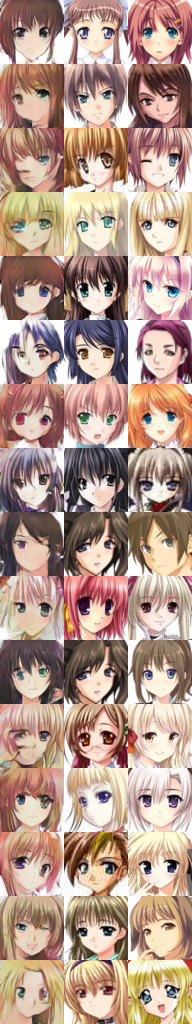
\includegraphics[height=.69\textheight]{A2_dcgan_diffaugment_nearest_neighbors.png}\caption{Mỗi hàng: generated, nearest train, nearest test trong feature Inception;16 ảnh sinh đầu tiên, DiffAugment.}\label{fig:neighbors}\end{figure}
Đây là chẩn đoán trong không gian feature, không phải tìm theo pixel. Code giới hạn pool train tham chiếu ở 5.000 ảnh đầu được extract, test 5.000 ảnh; vì vậy không gọi là nearest neighbor trên toàn bộ 34.522 train. Chỉ 16 ảnh sinh được hiển thị. Có ảnh gần nhau không đủ kết luận memorization; không thấy bản sao cũng không chứng minh không memorize.

Hướng kiểm tra tiếp là tìm lân cận trên toàn bộ train và dùng thêm pixel/perceptual distance với ngưỡng đăng ký trước. Near-duplicate khác crop vẫn có thể qua exact dedup; các thí nghiệm đó chưa được thực hiện trong báo cáo này.
\clearpage

\section{Hạn chế, kết luận và tái lập}\label{sec:limits}
Đây là study hai biến thể DCGAN, không so sánh GAN với diffusion và không tái lập BigGAN/StyleGAN2 của paper. Cùng seed không loại bỏ tính ngẫu nhiên hoặc ước lượng được phương sai qua lần train. KID subset std và IS split std không phải khoảng tin cậy multi-seed; chưa có kiểm định ý nghĩa thống kê.

Extractor ImageNet có thể không bắt hết sai lệch khuôn mặt anime; số mẫu 5.000 hữu hạn. Exact dedup không loại near-duplicate; split không phân tầng theo nhân vật. Policy gộp ba thành phần nên chưa quy kết được tác động riêng. Final EMA được cố định ở 20.000 updates, không chứng minh hội tụ. Grid/nearest neighbor chỉ là chẩn đoán, không bảo chứng không sao chép dữ liệu.

Kết luận được hỗ trợ là DiffAugment cải thiện mạnh so với baseline ở recipe này, nhưng recall còn thấp và lỗi thị giác vẫn có. Bước tiếp nên lặp nhiều seed, ablate policy, tăng độ chặt chẽ của kiểm tra memorization và đánh giá human perception, thay vì chỉ tối ưu FID. Không cộng các kế hoạch đó vào kết quả đã đạt.

\subsection{Tái lập và kiểm toán}\label{sec:repro}
Notebook nguồn \path{A2/a2_dcgan_diffaugment.ipynb}; notebook đã chạy \path{A2/dcgan-vs-augmenteddcgan-dl-assignment-2.ipynb}. Bundle \path{artifacts/A2/} giữ config, environment, metric protocol, full history 20.000 dòng/variant và hình. Website gộp history để hiển thị; bảng báo cáo dùng artifact gốc, không dùng preview hoặc nội suy dữ liệu.

\path{python tools/prepare_reports.py} kiểm tra hash bundle và ngân sách, sinh bảng/hình và provenance. Source validation checkpoint được ghi ở lần pack gốc; không mô tả như lần biên soạn này nạp checkpoint đã loại khỏi bundle. \path{python tools/build_reports.py} build PDF không cần ML libraries/GPU/raw dataset. Video và xác nhận các mốc nộp bài vẫn là phần cần hoàn thiện trước khi nộp.
\clearpage
\bibliographystyle{plain}\bibliography{shared/references}
\clearpage\appendix
\section{Nearest neighbors của baseline}
\begin{figure}[H]\centering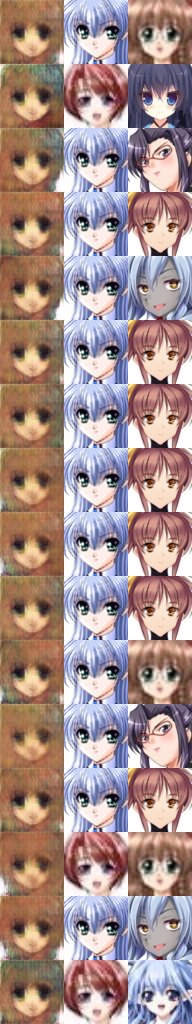
\includegraphics[height=.74\textheight]{A2_dcgan_baseline_nearest_neighbors.png}\caption{Baseline: generated/nearest train/nearest test với cùng giới hạn pool tham chiếu. Lặp mẫu quan sát được phải xem cùng recall 0 và FID 298,51.}\label{fig:bneighbors}\end{figure}
\end{document}